\documentclass[11pt, a4paper]{article}
\usepackage[utf8]{inputenc}

\usepackage[margin=1in]{geometry} 
\usepackage{amsmath,amsthm,amssymb}
\usepackage[margin=1in]{geometry} 
\usepackage{amsmath,amsthm,amssymb}

\usepackage[slovene]{babel}
\usepackage{color}
\usepackage{graphicx}
\usepackage{amssymb}
\usepackage{amsmath}
\usepackage{mathtools}
\usepackage{commath}
\usepackage{ragged2e}
\usepackage[T1]{fontenc}
\usepackage[normalem]{ulem}
\usepackage{amsthm}
\usepackage{esvect}
\usepackage{float}
\usepackage{calrsfs}
\DeclareMathAlphabet{\pazocal}{OMS}{zplm}{m}{n}
\newcommand{\Ga}{\mathcal{G}}
\mathtoolsset{showonlyrefs} 

\newcommand\setItemnumber[1]{\setcounter{enumi}{\numexpr#1-1\relax}}


\newtheorem{theorem}{Trditev}[section]
\newtheorem{corollary}{Posledica}[section]
\newtheorem{lemma}[section]{Lema}
\theoremstyle{definition}
\newtheorem{definition}{Definicija}[section]
\theoremstyle{example}
\newtheorem{example}[section]{Primer}
\theoremstyle{izrek}
\newtheorem{izrek}[section]{Izrek}

\begin{document}
\begin{center}
\thispagestyle{empty}
\parskip=14pt%
\vspace*{3\parskip}%
\begin{Huge} Sklopljeni nihajni krog \end{Huge}

By

Matic Tonin

ID No. (28181098)

Mentor 

(Rok Dolenc)

\rule{7cm}{0.4pt}

Pod okvirom:

FAKULTETE ZA FIZIKO IN MATEMATIKO, LJUBLJANA

22. 3. 2020

\end{center}
\pagebreak
\section{Naloga}
\begin{enumerate}
\item Izmeri casovni potek napetosti na obeh krogih pri vzbujanju s stopnicastim signalom za vse razliène sklopitve $C_{0}[\mathrm{pF}]=0,150,330,560,820,1150$.
\item Izmeri frekvenčno karakteristiko enega nihajnega kroga in določi $Q$.
\item Izmeri frekvenèno karakteristiko skloplienih nihajnih krogov z meritvijo odziva drugega kroga za vsak $C_{0}$ in izmeri razliko lastnih kroãnih frekvenc $\Delta \omega$.
\end{enumerate}
\section{Meritve}
\subsection{Časovni potek napetosti}
\textbf{\underline{$C_0=0 pF$}}\\

\begin{figure}[htp]
    \centering
    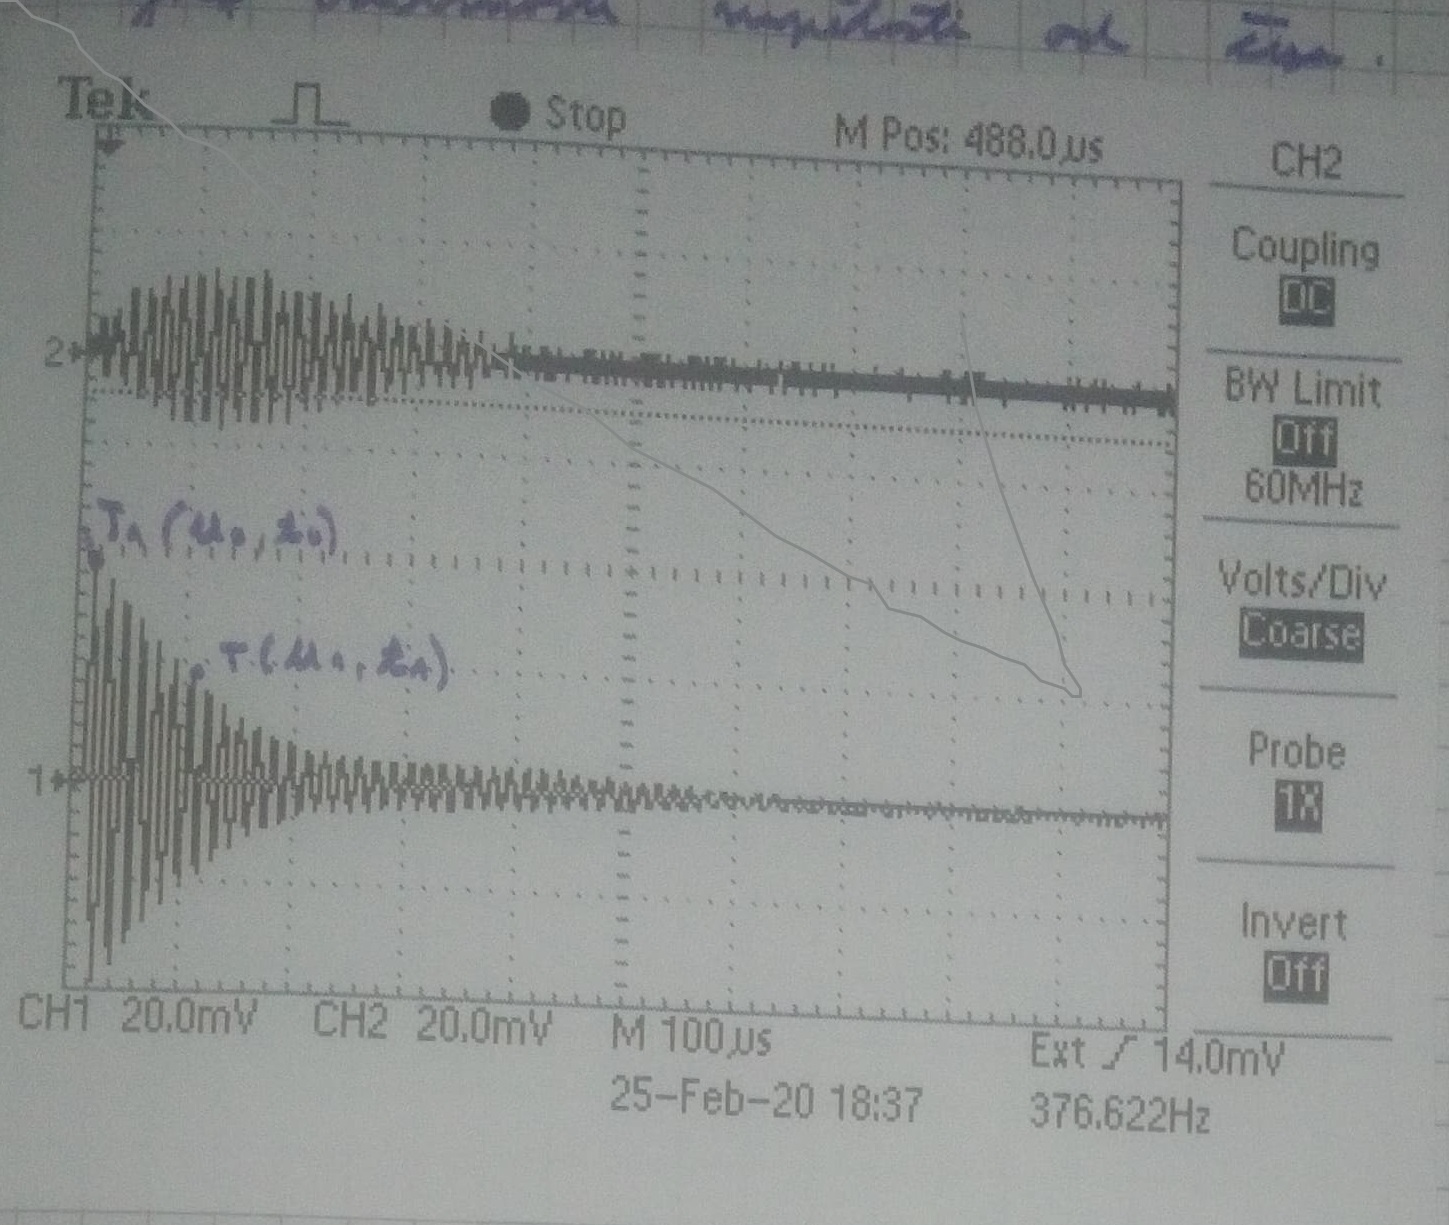
\includegraphics[width=10cm]{C=0.jpg}
    \caption{Graf napetosti v odvisnosti od časa, $C_0=0 pF$}
\end{figure}
Za ta del vaje smo potrebovali najprej izmeriti, koliko je lastna frekvenca nihanja nihajnega kroga, ko nastavimo kapacitivnost kondenzatorja $C_0=0 pF$.
Za to uporabimo enačbo: $$\underline{\underline{\omega}}=\frac{N}{t}=\frac{10}{150\mu s}=\underline{\underline{0.06 \frac{1}{\mu s}}}$$
Pri čemer je N število nihajev v časovnem intervalu t. 
Manjka nam samo še koeficient $\beta$, ki pa ga dobimo z obračanjem enačb:
$$U_1=U_0e^{-\beta t}\cos(\omega t)$$
Iz česar nam sledi, da je koeficient dušenja enak kar:
$$ \beta=\ln\left(\frac{U_1}{U_0}\right)\cdot t^{-1}=\underline{\underline{5500\frac{1}{s}}}$$
Te dve vrednosti se v poteku naše meritve ne spreminjata, saj sta to karakteristične vrednosti za naš 1. nihajni krog. 

\pagebreak
\textbf{\underline{$C_0=150pF$}}\\

\begin{figure}[htp]
    \centering
    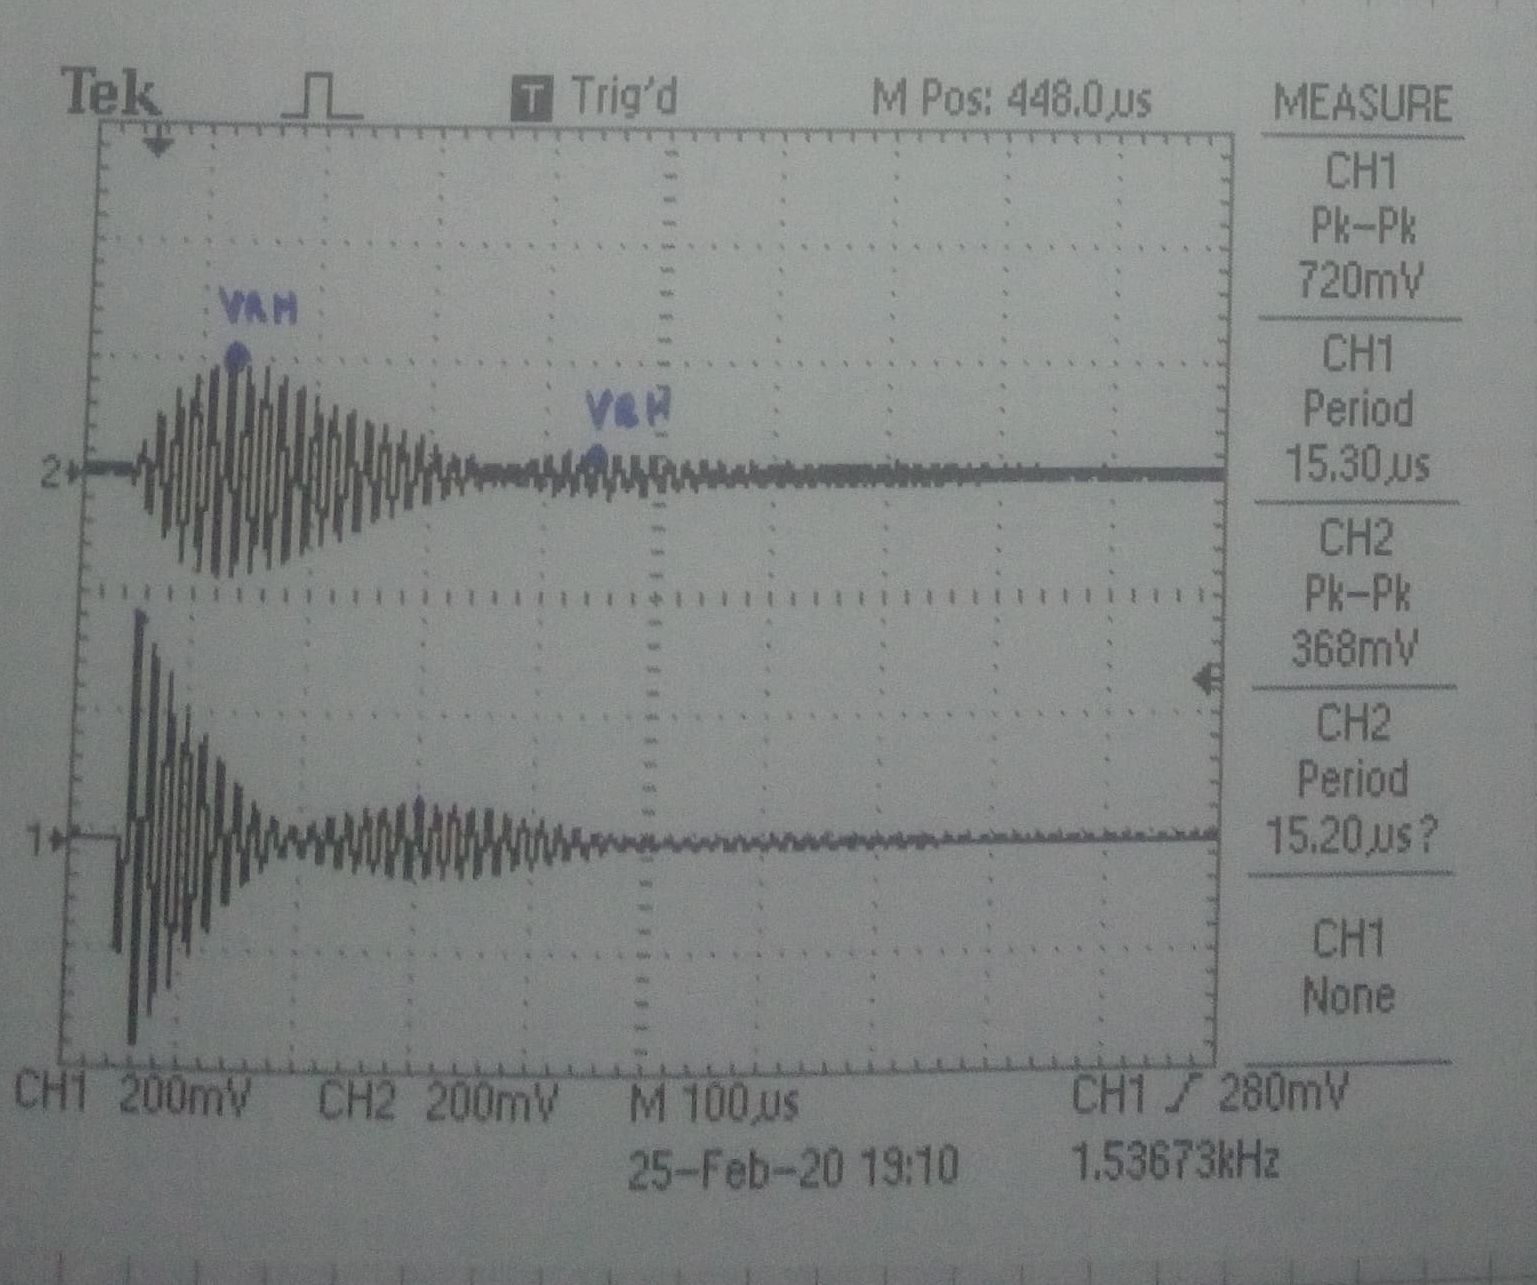
\includegraphics[width=10cm]{C=150.jpg}
    \caption{Graf napetosti v odvisnosti od časa, $C_0=150 pF$}
\end{figure}
Ker v tem primeru naša kapacitivnost 2 kondenzatorja ni več enaka nič, moramo uporabiti druge enačbe in sicer: 
$$\cos\left(\frac{\Delta \omega_{1,2}}{2}t\right)=\frac{U_{1,2}}{U_0}e^{\beta t}$$
Reševanje tega problema si lahko rahlo poenostavimo, če merimo dva vrhova našega utripanja.
Če na naši sliki izberemo zgolj maksimume v utripanju, lahko izmerimo s tem frekvenco utripanja prvega in drugega nihajnega kroga.
Tako se nam enačba poenostavi v:
$$\Delta \omega_{1,2}=\arccos \left(\frac{U_{1,2}}{U_0}\right) \frac{2}{t} $$
Kjer je t perioda med dvema vrhovoma.\\
Tako lahko za naše izbrane vrednosti izračunamo, koliko je krožna frekvenca utripanja za kapacitivnost kondenzatorja z $C_0=150pF$.\\
Torej za moj primer je to bilo: \\

\begin{table}[ht]
	\centering
	\begin{tabular}{|c|c|c|c|c|}
		\hline
		Nihajni krog & $U_i$ & $U_0$ & $ t_i$ & $\Delta \omega_i$ \\
		\hline
		\hline
		1 & 50 & 360 & 320$pF$ & 408.5 Hz \\
		\hline
		2 & 20 & 200 & 320$pF$ & 312.5 Hz \\
		\hline
		\end{tabular}
		\caption{Prikaz meritev pri $C_0=150pF$}
		\label{tab:FirstTable}
\end{table}

\pagebreak
\textbf{\underline{$C_0=330pF$}}\\

\begin{figure}[htp]
    \centering
    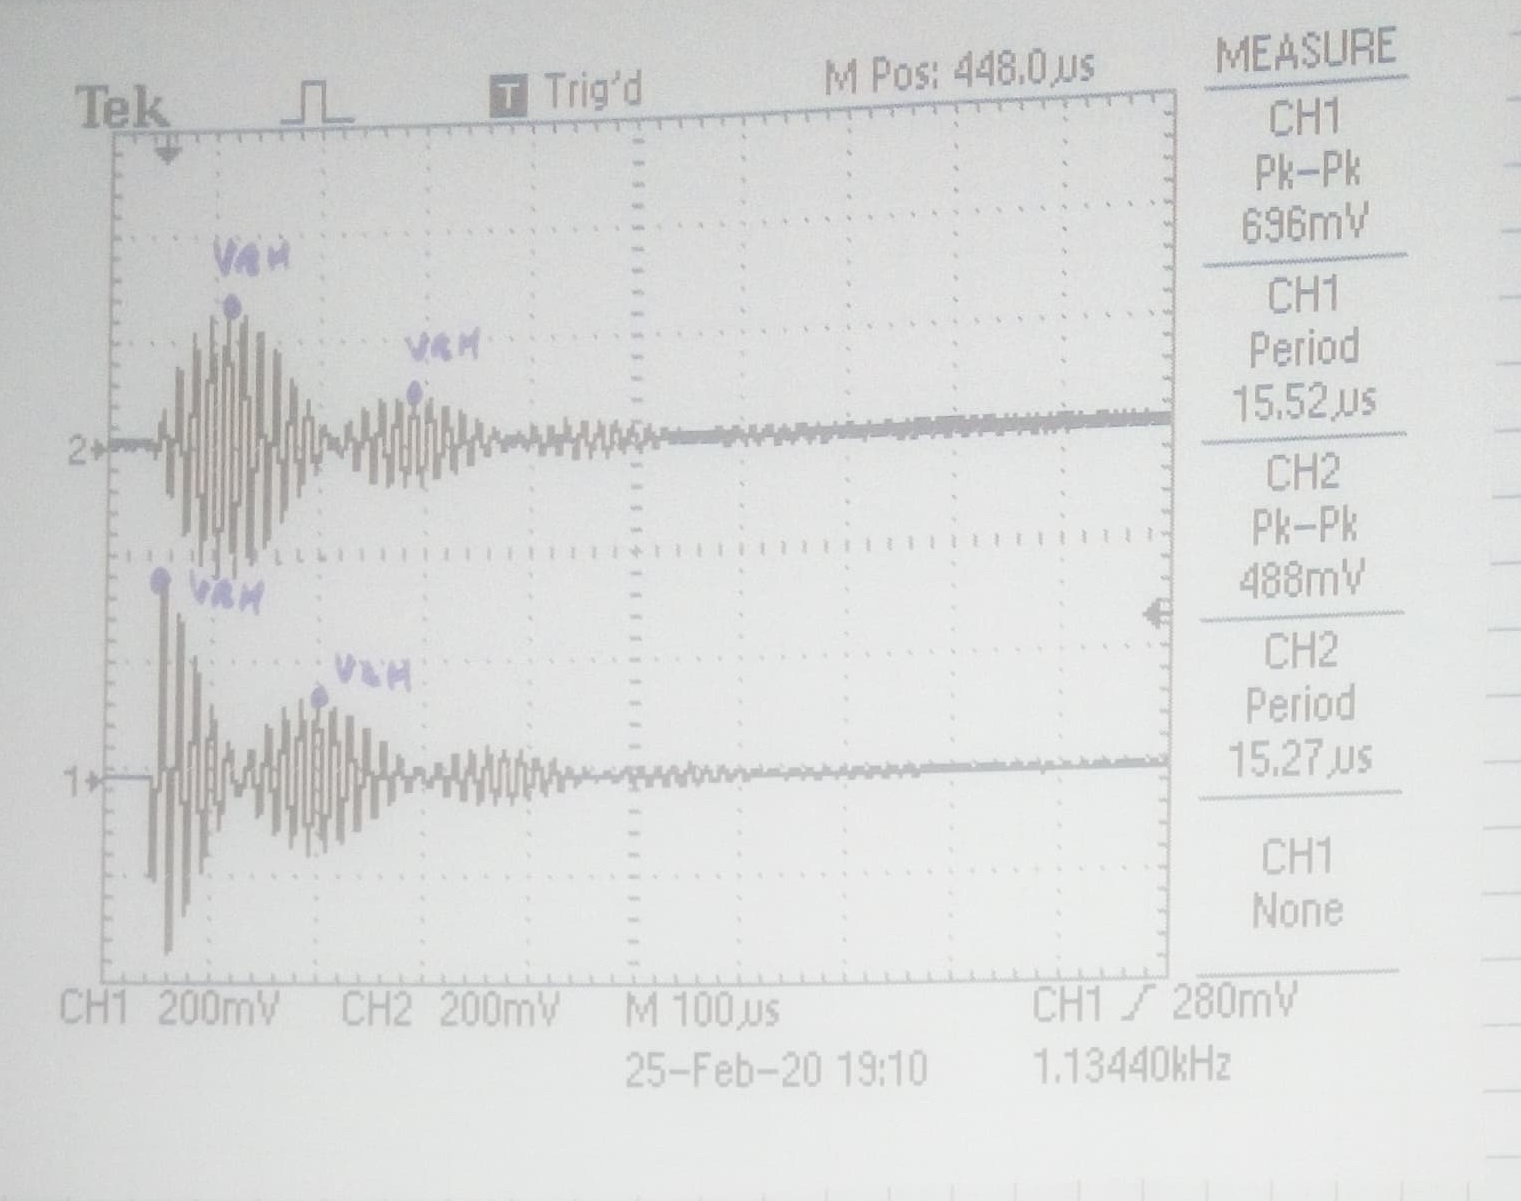
\includegraphics[width=10cm]{C=330.jpg}
    \caption{Graf napetosti v odvisnosti od časa, $C_0=330 pF$}
\end{figure}

Pri tem delu bomo uporabili podoben princip, kot pri poglavju za $C_0=150pF$. Torej bomo ponovno uporablili enačbo:
$$\Delta \omega_{1,2}=\frac{U_{1,2}}{U_0}\frac{1}{t} $$
Kjer je t perioda med dvema vrhovoma.\\
Torej za moj primer je to bilo: \\
\begin{table}[ht]
	\centering
	\begin{tabular}{|c|c|c|c|c|}
		\hline
		Nihajni krog & $U_i$ & $U_0$ & $ t_i$ & $\Delta \omega_i$ \\
		\hline
		\hline
		1 & 120 & 360 & 140$pF$ & 2380 Hz \\
		\hline
		2 & 80 & 270 & 160$pF$ & 1851 Hz \\
		\hline
		\end{tabular}
		\caption{Prikaz meritev pri $C_0=330pF$}
		\label{tab:FirstTable}
\end{table}

\pagebreak
\textbf{\underline{$C_0=520pF$}}\\

\begin{figure}[htp]
    \centering
    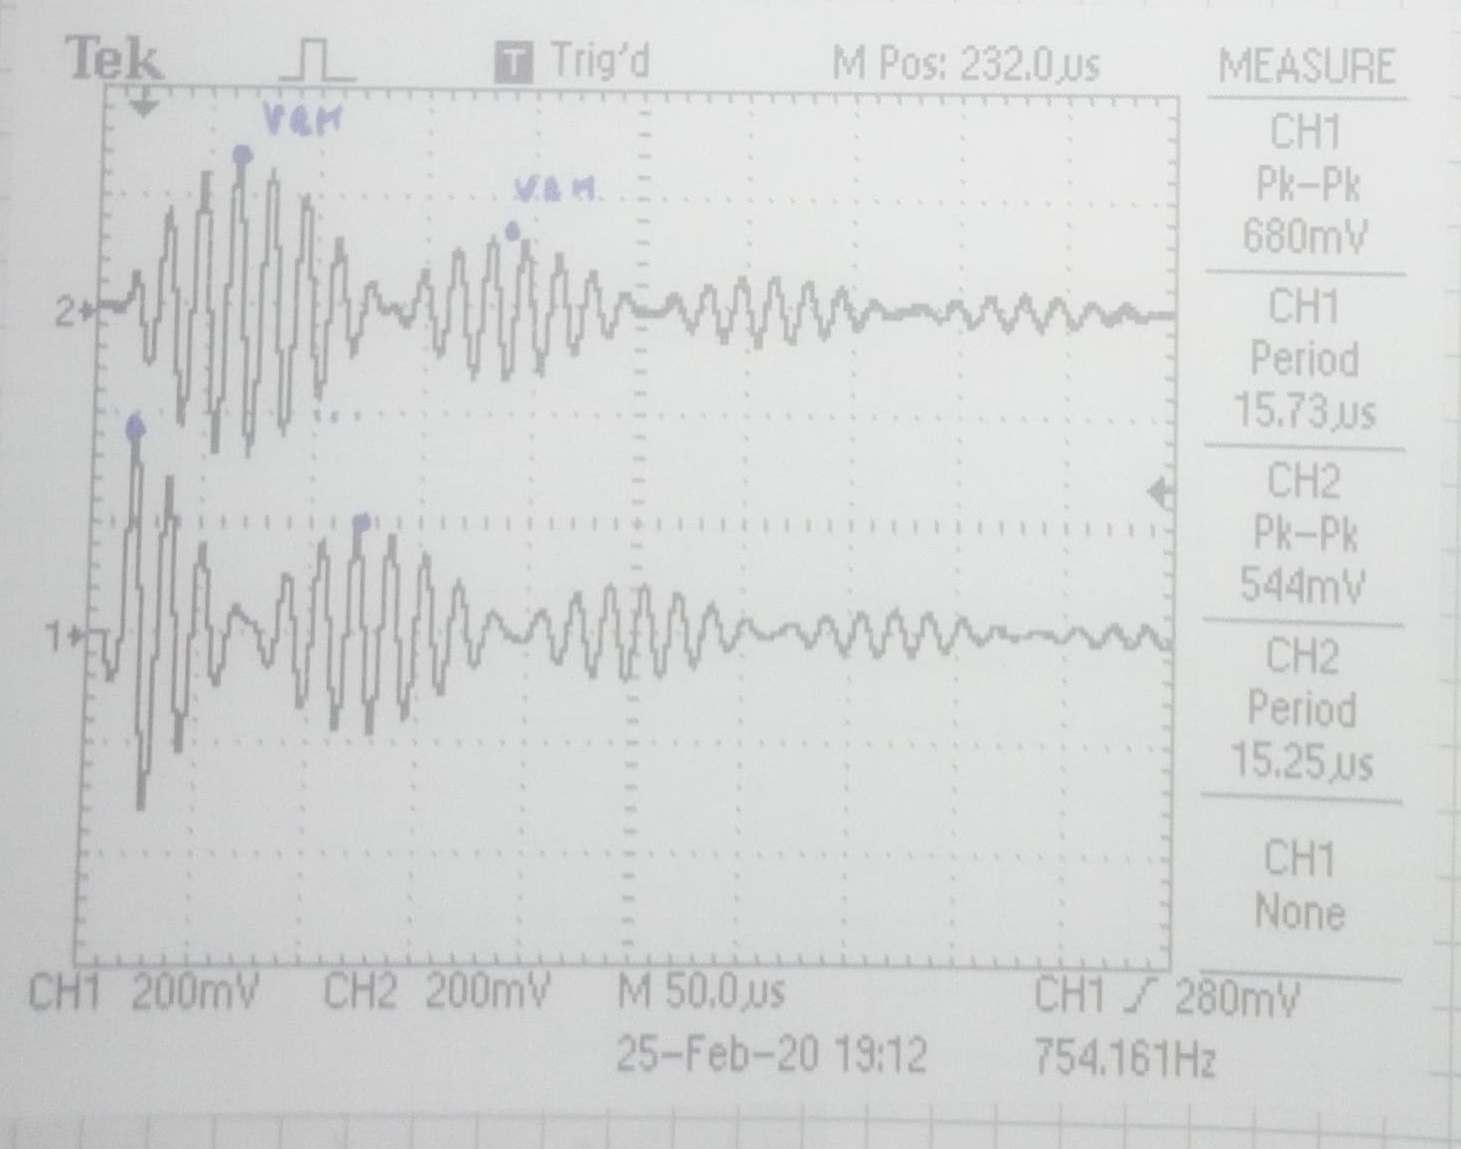
\includegraphics[width=10cm]{C=520.jpg}
    \caption{Graf napetosti v odvisnosti od časa, $C_0=520 pF$}
\end{figure}

Pri tem delu bomo uporabili podoben princip, kot pri poglavju za $C_0=150pF$. Torej bomo ponovno uporablili enačbo:
$$\Delta \omega_{1,2}=\frac{U_{1,2}}{U_0}\frac{1}{t} $$
Kjer je t perioda med dvema vrhovoma.\\
Torej za moj primer je to bilo: \\
\begin{table}[ht]
	\centering
	\begin{tabular}{|c|c|c|c|c|}
		\hline
		Nihajni krog & $U_i$ & $U_0$ & $ t_i$ & $\Delta \omega_i$ \\
		\hline
		\hline
		1 & 200 & 360 & 110$pF$ & 5050 Hz \\
		\hline
		2 & 120 & 270 & 130$pF$ & 3418 Hz \\
		\hline
		\end{tabular}
		\caption{Prikaz meritev pri $C_0=520pF$}
		\label{tab:FirstTable}
\end{table}

\pagebreak
\textbf{\underline{$C_0=820pF$}}\\

\begin{figure}[htp]
    \centering
    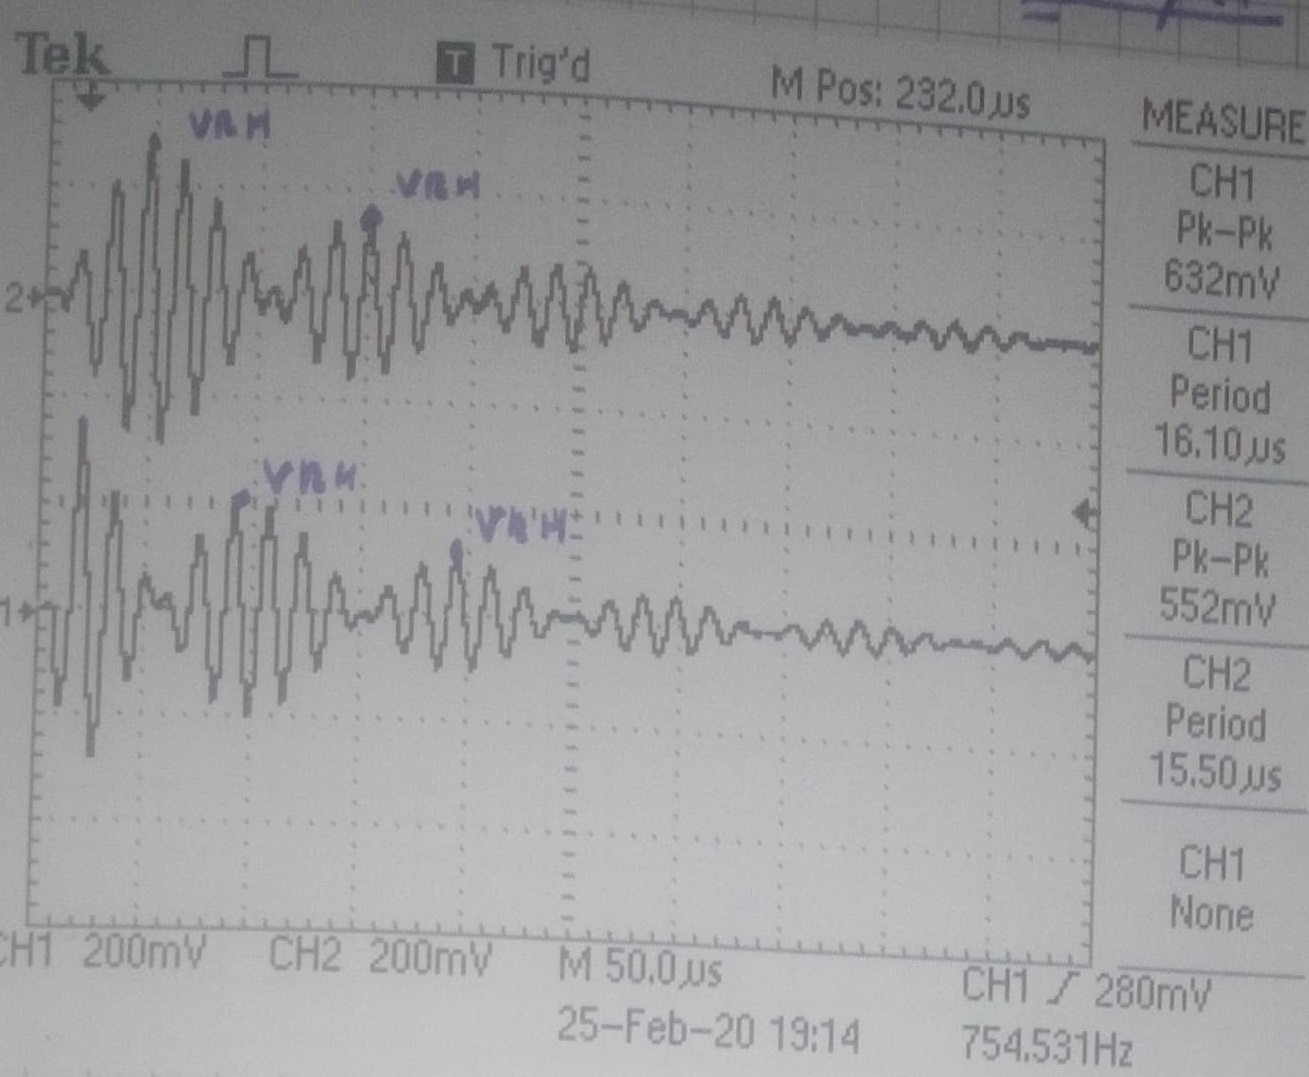
\includegraphics[width=10cm]{820.jpg}
    \caption{Graf napetosti v odvisnosti od časa, $C_0=820 pF$}
\end{figure}

Pri tem delu bomo uporabili podoben princip, kot pri poglavju za $C_0=150pF$. Torej bomo ponovno uporablili enačbo:
$$\Delta \omega_{1,2}=\frac{U_{1,2}}{U_0}\frac{1}{t} $$
Kjer je t perioda med dvema vrhovoma.\\
Torej za moj primer je to bilo: \\
\begin{table}[ht]
	\centering
	\begin{tabular}{|c|c|c|c|c|}
		\hline
		Nihajni krog & $U_i$ & $U_0$ & $ t_i$ & $\Delta \omega_i$ \\
		\hline
		\hline
		1 & 200 & 360 & 70$pF$ & 7936 Hz \\
		\hline
		2 & 160 & 280 & 100$pF$ & 5714 Hz \\
		\hline
		\end{tabular}
		\caption{Prikaz meritev pri $C_0=820pF$}
		\label{tab:FirstTable}
\end{table}

\pagebreak
\textbf{\underline{$C_0=1100pF$}}\\

\begin{figure}[htp]
    \centering
    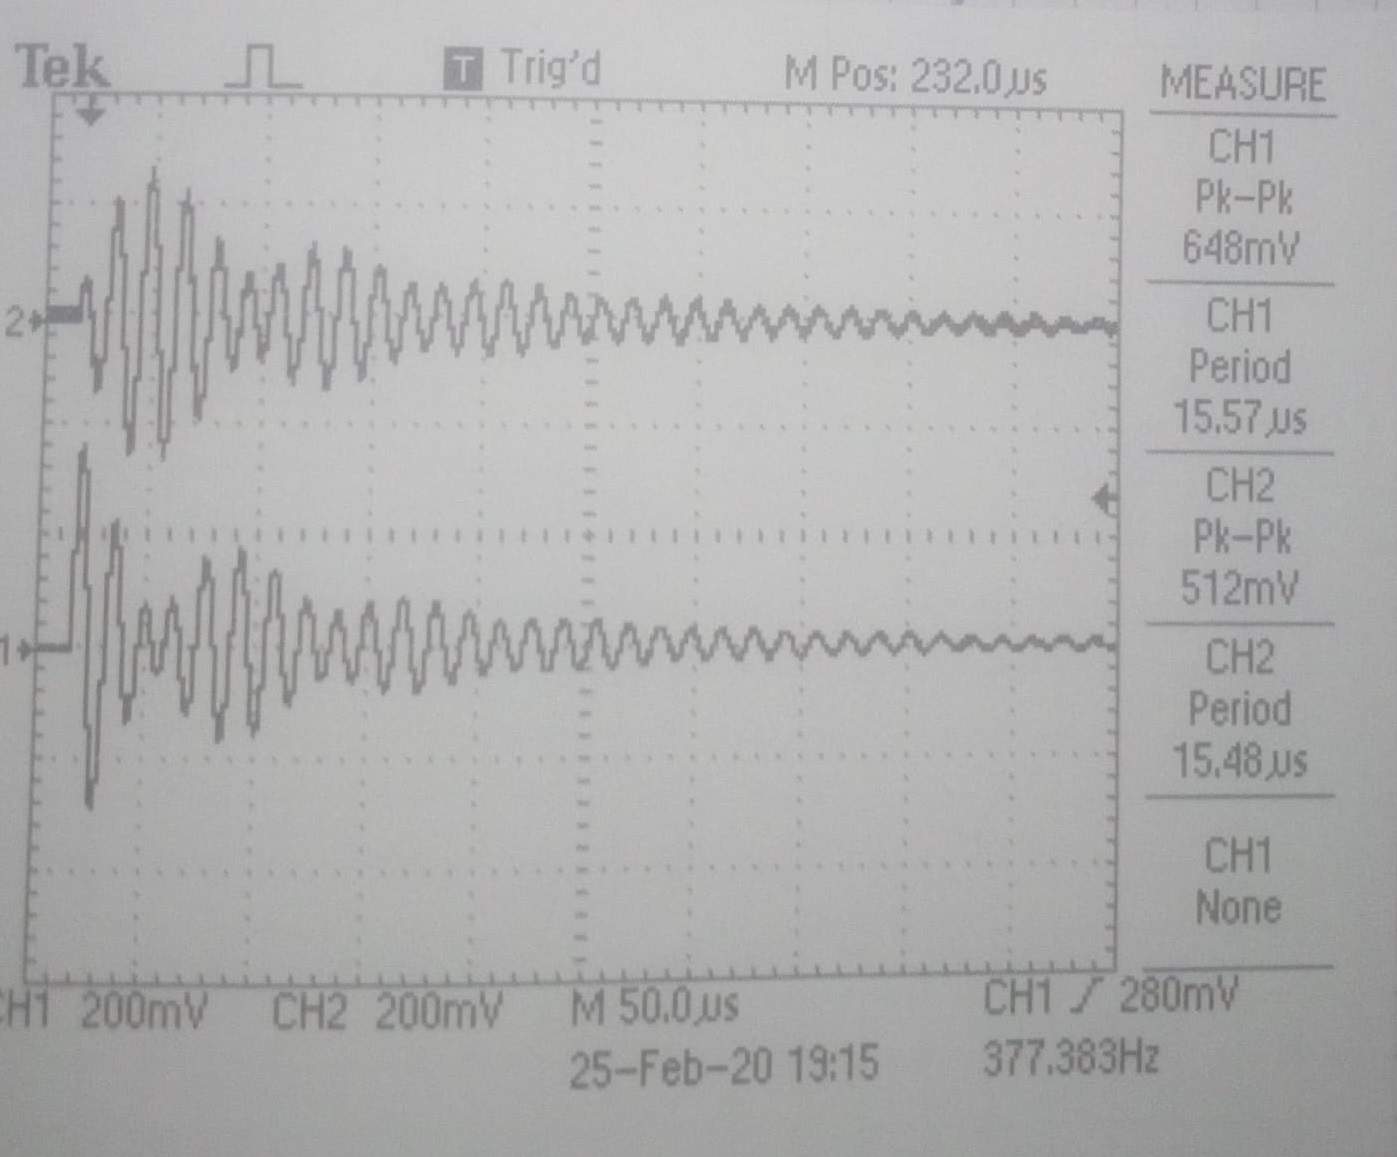
\includegraphics[width=10cm]{C=1100.jpg}
    \caption{Graf napetosti v odvisnosti od časa, $C_0=1100 pF$}
\end{figure}

Pri tem delu bomo uporabili podoben princip, kot pri poglavju za $C_0=150pF$. Torej bomo ponovno uporablili enačbo:
$$\Delta \omega_{1,2}=\frac{U_{1,2}}{U_0}\frac{1}{t} $$
Kjer je t perioda med dvema vrhovoma.\\
Torej za moj primer je to bilo: \\
\begin{table}[ht]
	\centering
	\begin{tabular}{|c|c|c|c|c|}
		\hline
		Nihajni krog & $U_i$ & $U_0$ & $ t_i$ & $\Delta \omega_i$ \\
		\hline
		\hline
		1 & 200 & 360 & 80$pF$ & 6944 Hz \\
		\hline
		2 & 120 & 280 & 70$pF$ & 6122 Hz \\
		\hline
		\end{tabular}
		\caption{Prikaz meritev pri $C_0=1100pF$}
		\label{tab:FirstTable}
\end{table}

\pagebreak
\subsection{Frekvenčna karakteristika enega kroga}
Za frekvenčno karakteristiko smo merili velikosti posameznih amplitud pri različnih vrednostih vsiljene frekvence. Z merjenjem smo začeli pri vrednosti 50kHz in nato počasi dvigali vrednosti vse do 90 Hz. Pri tem smo opazovali, kako se na našo vsiljeno frekvenco odziva en in drug nihajni krog. \\
\begin{table}[ht]
	\centering
	\begin{tabular}{|c|c|c|c|c|}
		\hline
		$\omega$ & $2U_1$ & $2U_2$ \\
		\hline
		\hline
		50 & 0.864 & 0.088 \\
		\hline
		55 & 1.32 & 0.144 \\
		\hline
		60 & 2.64 & 0.40 \\
		\hline
		63 & 4.42 & 0.88 \\
		\hline
		65 & 9.84 & 3.64 \\
		\hline
		\hline
		66.23 & 11.5 & 8.08 \\
		\hline
		\hline
		68 & 7.60 & 4.8 \\
		\hline
		70 & 4.36 & 1.34 \\
		\hline
		75 & 2.38 & 0.42 \\
		\hline
		80 & 1.54 & 0.18 \\
		\hline
		85 & 1.18 & 0.140 \\
		\hline
		90 & 0.968 & 0.1 \\
		\hline
		\end{tabular}
		\caption{Tabela meritev odziva amplitude v odvisnosti od vsiljene frekvence }
		\label{tab:FirstTable}
\end{table}

In vidimo, da se maksimum pojavi pri 66,23 Hz in sicer na krogu 1 z amplitudo 6.25V na 2 pa z amplitudo 4.04V.\\
\begin{figure}[htp]
    \centering
    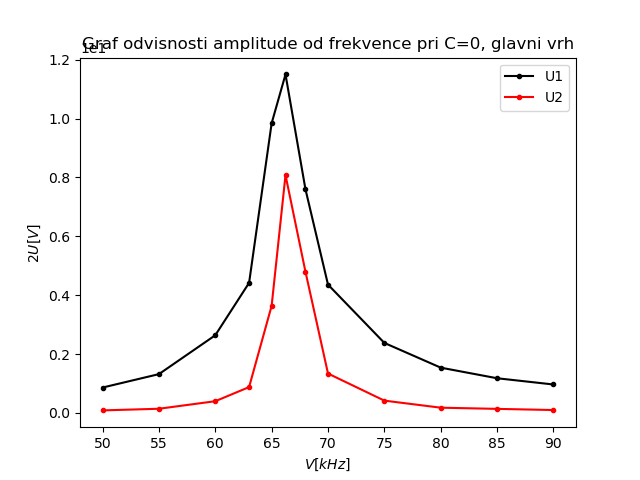
\includegraphics[width=12cm]{Karakteristika za C=0.png}
    \caption{Graf napetosti v odvisnosti od vsiljene frekvence, $C_0=0 pF$}
\end{figure}

\pagebreak
\underline{Sedaj nas zanima še, koliko je Q.} \\
\medskip

Q smo definirali kot $$Q=\frac{\omega_0}{\Delta \omega}$$
kjer je $\Delta \omega$ podana kot širina resonančnega odziva $2\beta$, ko merimo med točkama, kjer pade napetost za faktor $\sqrt{\frac{1}{2}}=0,70$ od maksimalne vrednosti.
Kako smo to izvedli na naši meritvi. Najprej smo pogledali, koliko sta maksimuma meritve, ju pomnožili z našim faktorjem $\sqrt{\frac{1}{2}}=0,70$ in poiskali, na kateri frekvenci se je pojavila ta številka:
\begin{table}[ht]
	\centering
	\begin{tabular}{|c|c|c|c|}
		\hline
		Nihajni krog & $U_{max}[V]$ & $\sqrt{\frac{1}{2}} U_{max}[V]$ & $\omega_i$ [kHz]\\
		\hline
		\hline
		1 & 6.25 & 4.41 & 64.67\\
		\hline
		2 &  4.04 & 2.87 & 65.31 \\
		\hline
		\end{tabular}
		\caption{Prikaz meritev maksimalne frekvence in odmika v nihajnem krogu.}
		\label{tab:FirstTable}
\end{table}

Iz naše tabele pa lahko razberemo, da je $\Delta \omega=0.64 kHz$

Torej lahko zapišemo, da je koeficient $\Delta \omega$ kar enak:
$$\frac{\Delta \omega}{2}= \beta =0.35 kHz$$

S tem smo dobili vse potrebno za izračun našega Q
$$\underline{\underline{Q}} =\frac{\omega_0}{\Delta \omega}=\frac{60000}{350}=\underline{\underline{171.42}} $$

\pagebreak
\subsection{Frekvenčna karakteristika sklopljenih krogov z meritvijo odziva}

Pri tem delu vaje mo osciloskop preklopili tako, da je kazal sklopitev obeh valov na enkrat in nato merili, kakšen je odziv amplitude sklopljenega kroga od vsiljene frekvence pri vseh kapacitivnosti. Te meritve smo nato nanizali na skupen graf in videli, kaj se dogaja. \\
Na žalost, zaradi pomanjkanja časa ob koncu vaje, moje meritve ob prvih vrhovih niso bile idealne in se zato ne vidi popolno, kako bi se morali počasi vrhovi z višanjem kapacitivnosti nižati. \\

\begin{figure}[htp]
    \centering
    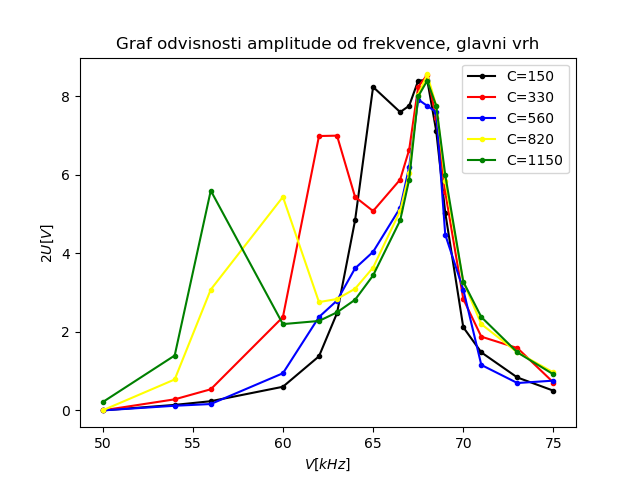
\includegraphics[width=12cm]{Graf odvisnosti amplitude od frekvence ožji.png}
    \caption{Graf karakteristike sklopljenih krogov, narejen graf}
\end{figure}

Kako točno bi moralo zgledati pa nam pokaže naslednja slika.

\begin{figure}[htp]
    \centering
    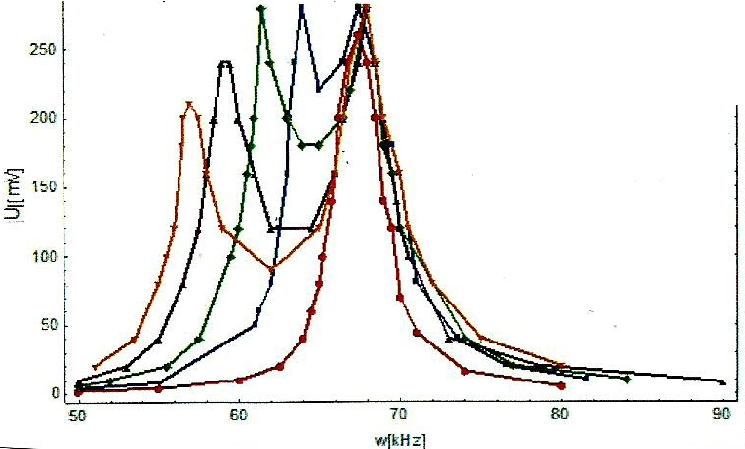
\includegraphics[width=12cm]{Pravilna meritev.png}
    \caption{Graf karakteristike sklopljenih krogov, pravilen graf, avtor Anonimen}
\end{figure}

Meritve, ki sem jih izmeril bom poslal v dodatni datoteki. 

\pagebreak
\section{Napake}
\subsection{Časovni potek napetosti}
Pri tem delu se je pojavljala napaka večinsko zaradi odčitavanja podatkov iz meritev in to napako ocenjujem, da je:
\begin{center}
$\Delta$ $U =5 mV$\quad in \quad $\Delta$ $t=10 \mu s$
\end{center}  
Tako so napake meritev:
\begin{table}[ht]
	\centering
	\begin{tabular}{|c|c|c|c|c|c|c|}
		\hline
		$C_0$ [pF] & $\delta U_1$ & $\delta U_2$ & $U_0$ & $\delta t$ & Skupna relativna napaka 1. &Skupna relativna napaka 2.\\
		\hline
		\hline
		150 & 0.1 & 0.25 & 0.138 & 0.06225 & 0.38125 & 0.270 \\
		\hline
		330 & 0.04 & 0.0625 & 0.138 & 0.03125 & 0.21 & 0.231 \\
		\hline
		520 & 0.05 & 0.0833 & 0.138 & 0.077 & 0.258 & 0.2913 \\
		\hline
		520 & 0.05 & 0.0833 & 0.138 & 0.077 & 0.258 & 0.2913 \\
		\hline
		820 & 0.05 & 0.0833 & 0.138 & 0.1& 0.288 & 0.3213 \\
		\hline
		1120 & 0.05 & 0.0833 & 0.138 & 0.1& 0.258 & 0.2913 \\
		\hline
		\end{tabular}
		\caption{Prikaz napak pri meritvi vseh frekvenc}
		\label{tab:FirstTable}
\end{table}

\subsection{Frekvenčna karakteristika enega kroga}
V tem delu so se napake pojavile predvsem pri odčitavanju iz naprave ali pa zaradi napačnih nastavitev na napravi. To se naprimer dobro vidi na grafu karakteristike, kjer se bi morali dobiti resonančno funkcijo, ampak se moje vrednosti ne ujemajo popolnoma. Natančnost te meritve bi lahko izboljšali z povečanjem števila meritev na območju, kjer je to najbolj potrebno, na našem primeru v intervalu [62 kHz, 70 kHz], da bi se bolje videlo kako poteka vzpenjanje krivulje do vrha.

\subsection{Frekvenčna karakteristika sklopljenih krogov z meritvijo odziva}
Enak komentar kot pri prejšnjem poglavju bi lahko uporabili tudi tu. Več meritev na intervalih prvega vrha bi nam pomagale boljše določiti, kako se sklopljeno nihalo odziva na vsiljeno nihanje. 

\section{Rezultati}
\subsection{Časovni potek napetosti}
\begin{table}[ht]
	\centering
	\begin{tabular}{|c|c|c|c|c|c|c|}
		\hline
		$C_0$ [pF] & $\Delta \omega_1$ [Hz] & $\Delta \omega_2 $ [Hz] \\
		\hline
		\hline
		150 & 408.5 & 312.5  \\
		\hline
		330 & 2380 & 1851  \\
		\hline
		520 & 5050 & 3418\\
		\hline
		820 & 7936 & 5714 \\
		\hline
		1120 & 6944 & 6122\\
		\hline
		\end{tabular}
		\caption{Prikaz napak pri meritvi vseh frekvenc}
		\label{tab:FirstTable}
\end{table}

\subsection{Frekvenčna karakteristika enega kroga}

\begin{figure}[htp]
    \centering
    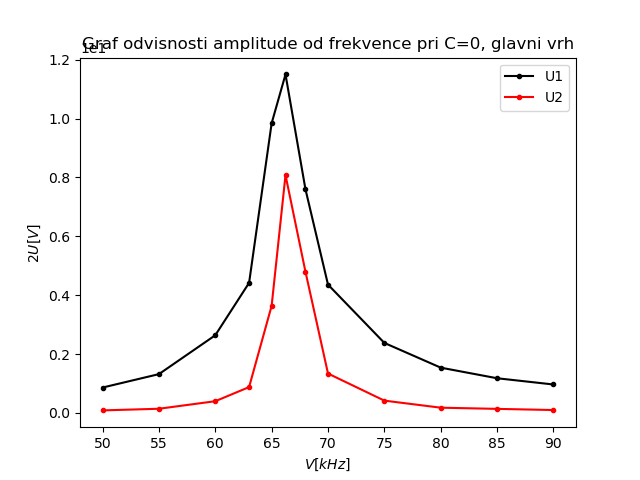
\includegraphics[width=12cm]{Karakteristika za C=0.png}
    \caption{Graf napetosti v odvisnosti od vsiljene frekvence, $C_0=0 pF$}
\end{figure}

\subsection{Frekvenčna karakteristika sklopljenih krogov z meritvijo odziva}

\begin{figure}[htp]
    \centering
    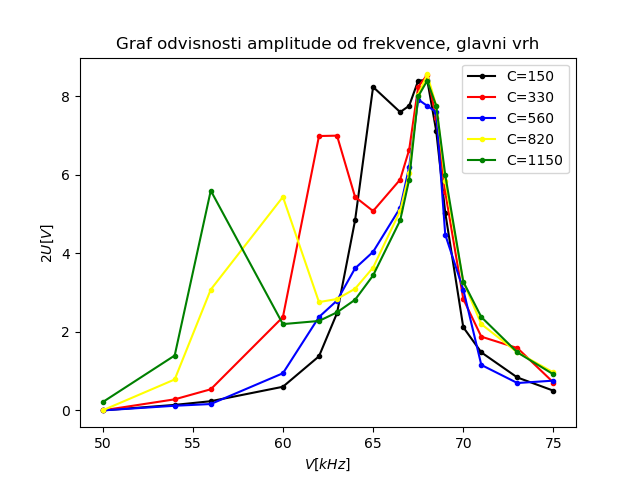
\includegraphics[width=12cm]{Graf odvisnosti amplitude od frekvence ožji.png}
    \caption{Graf karakteristike sklopljenih krogov, narejen graf}
\end{figure}

\end{document}